\appendixprefix

\section{Implementation of View Encoders}
\label{supp:view-encoders}

In this section, we introduce the detailed implementation of the four view encoders.
We denote the representation for node (atom) \(v_i\) as \(\bm{h}_i\) and the representation at the graph (molecule) level as \(\bm{z}\).
As each encoder is independent to each other, we omit the superscript representing the specific view \(m \in \{\text{2D}, \text{3D}, \text{FP}, \text{SM}\}\) is clear for notation simplicity.
Also, for clarity, when the context is clear, we omit the subscript \(j\) that indexes the molecule.

\paragraph{Embedding 2D graphs.}
Graph Isomorphism Network (GIN) \cite{Xu:2019ty} is a simple and effective model to learn discriminative graph representations, which is proved to have the same representational power as the Weisfeiler-Lehman test \cite{Weisfeiler:1968wl}.
Since GIN has been widely adopted for 2D graph representation learning \cite{Hu:2020uz,You:2021wl,You:2020ut}, we leverage a GIN model to obtain the representations for the 2D molecular graphs.
Recall that each molecule is represented as \(\mathcal{G} = (\bm{A}, \bm{X}, \tens{E})\), where \(\bm{A}\) is the adjacency matrix, \(\bm{X}\) and \(\tens{E}\) are features for atoms and bonds respectively.
The layer-wise propagation rule of GIN can be written as:
\begin{equation}
	\bm{h}_i^{(k + 1)} = f_{\text{atom}}^{(k+1)}\left(
	\bm{h}_i^{(k)} + \sum_{j \in\mathcal{N}(i)}
	\left(\bm{h}_j^{(k)} + f_{\text{bond}}^{(k+1)}(\etens{E}_{ij}))
	\right)\right),
\end{equation}
where the input features \(\bm{h}^{(0)}_i = \bm{x}_i\), \(\mathcal{N}(i)\) is the neighborhood set of atom \(v_i\), and \(f_{\text{atom}}, f_{\text{bond}}\) are two MultiLayer Perceptron (MLP) layers for transforming atoms and bonds features, respectively.
By stacking \(K\) layers, we can incorporate $K$-hop neighborhood information into each center atom in the molecular graph.
Then, we take the output of the last layer as the atom representations and further use the mean pooling to get the graph-level molecular representation:
\begin{equation}
\bm{z}^\text{2D} = \frac{1}{N}\sum_{i\in \mathcal{V}}\bm{h}_i^{(K)}.
\end{equation}



\paragraph{Embedding 3D graphs.}
Following GraphMVP \cite{Liu:2022vr}, we use the SchNet \cite{Schutt:2017wh} as the encoder for the 3D geometry graphs.
SchNet models message passing in the 3D space as continuous-filter convolutions, which is composed of a series of hidden layers, given as follows:
\begin{equation}
    \bm{h}_i^{(k + 1)} = f_\text{MLP}\left(\sum_{j=1}^N f_\text{FG}(\bm{h}_j^{(t)}, \bm{r}_i, \bm{r}_j)\right) + \bm{h}_i^{(t)},\\
\end{equation}
where the input \(\bm{h}^{(0)}_i = \bm{a}_i\) is an embedding dependent on the type of atom \(v_i\), \(f_\text{FG}(\cdot)\) denotes the filter-generating network. 
To ensure rotational invariance of a predicted property, the message passing function is restricted to depend only on rotationally invariant inputs such as distances, which satisfying the energy properties of rotational equivariance by construction.
Moreover, SchNet adopts radial basis functions to avoid highly correlated filters. The filter-generating network is defined as follow:
\begin{equation}
	f_\text{FG}(\bm{x}_j, \bm{r}_i, \bm{r}_j) = \bm{x}_j\cdot e_k(\bm{r}_i - \bm{r}_j) = \bm{x}_j \cdot \exp (-\gamma \|\|\bm{r}_i - \bm{r}_j\|_2 - \mu \|_2^2).
\end{equation}
Similarly, for non-quantum properties prediction concerned in this work, we take the average of the node representations as the 3D molecular embedding:
\begin{equation}
	\bm{z}^\text{3D} = \frac{1}{N}\sum_{i\in \mathcal{V}}\bm{h}_i^{(K)},
\end{equation}
where $K$ is the number of hidden layers.

\paragraph{Embedding fingerprints.}
Due to the discrete and extremely sparse nature of fingerprint vectors, we first transform all \(F\) binary feature fields into a dense embedding matrix \(\bm{F}' \in \mathbb{R}^{F \times D_\text{F}}\) via embedding lookup.
Then, we introduce a positional embedding matrix \(\bm{P} \in \mathbb{R}^{F \times D_\text{F}}\) to capture the positional relationship among bits in the fingerprint vector, which is defined as:
\begin{align}
	\bm{P}_{p, 2i} &= \sin(p/10000^{2i/D_F}),\\
	\bm{P}_{p, 2i+1} &= \cos(p/10000^{2i/D_F}),
\end{align}
where \(p\) denotes the corresponding bit position and \(i\) is corresponds to the \(i\)-th embedding dimension.
The positional embedding matrix will be added to the transformed embedding matrix:
\begin{equation}
	\bm{F} = \bm{F}' + \bm{P}.
\end{equation}
Thereafter, we use a multihead Transformer \cite{Vaswani:2017ul} to model the interaction among those feature fields.
Specifically, we first transform each feature into a new embedding space as:
\begin{align}
	\bm{Q}^{(h)} & = \bm{F}\bm{W}_\text{Q}^{(h)}, \\
	\bm{K}^{(h)} & = \bm{F}\bm{W}_\text{K}^{(h)}, \\
	\bm{V}^{(h)} & = \bm{F}\bm{W}_\text{V}^{(h)},
\end{align}
where the three linear transformation matrices \(\bm{W}_\text{Q}^{(h)}, \bm{W}_\text{K}^{(h)}, \bm{W}_\text{V}^{(h)} \in \mathbb{R}^{D_\text{F} \times \nicefrac{D}{H}}\) parameterize the query, key, and value transformations for the \(h\)-th attention head, respectively.
Following that, we compute the attention scores among all feature pairs and then linearly combine the value matrix from all \(H\) attention heads:
\begin{align}
	\bm{W}_\text{A}^{(h)} & = \operatorname{softmax}\left(\frac{\bm{Q}^{(h)}(\bm{K}^{(h)})^\top}{\sqrt{D_\text{H}}}\right), \\
	\widehat{\bm{Z}} & = \left[\bm{W}_\text{A}^{(1)}\bm{V}^{(1)} \,;\, \bm{W}_\text{A}^{(2)}\bm{V}^{(2)} \,;\, \dots \,;\, \bm{W}_\text{A}^{(H)}\bm{V}^{(H)} \right],
\end{align}
Finally, we perform sum pooling on the resulting embedding matrix \(\widehat{\bm{Z}} \in \mathbb{R}^{F \times D_\text{F}}\) and use a linear model \(f_\text{LIN}\) to obtain the final fingerprint embedding \(\bm{z}^\text{FP} \in \mathbb{R}^{D}\):
\begin{equation}
	\bm{z}^\text{FP} = f_\text{LIN} \left(\sum_{d=1}^{D_\text{F}} \widehat{\bm{Z}}_{d}\right).
\end{equation}

\paragraph{Embedding SMILES strings.}
Given ASCII-encoded SMILES strings, we first tokenize them with the Byte-Pair Encoder (BPE) tokenizer \cite{Gage:1994}, which strikes a balance among character- and word-level representations and allows to handle large vocabularies in molecular corpora.
Specifically, BPE finds the best word segmentation by iteratively and greedily merging frequent pairs of characters. In our implementation, we use a max vocabulary size of 52K tokens for both pretraining and downstream datasets.

After tokenization, we first pretrain a RoBERTa \cite{Liu:2019dd} model on the pretraining dataset with the masking language model as the sole training objective, as SMILES strings do not possess sequential relationships.
To be specific, $15\%$ tokens in a SMILES string are randomly selected and replaced with a special token \token{MASK}.
We also insert a special token \token{CLS} to each string to represent the whole molecule.
The training objective function is to independently predict the original tokens given the output on masked tokens.
Finally, the representation of the \token{CLS} token is regarded as the molecular embedding.

After pretraining the RoBERTa backbone, we freeze its parameters and leverage an additional MLP layer on top of each molecular embedding to obtain the final representation for each SMILES string.
This strategy improves memory efficiency and thus enables larger batch sizes for our contrastive pretraining framework.

\section{Dataset Description}
\label{supp:dataset}

In this section, we briefly introduce the datasets used for pretraining and fine-tuning, as well as details of dataset prepossessing.
Basic dataset statistics is summarized in \cref{tab:dataset}.

\begin{table}
	\centering
	\caption{Statistics of datasets used in experiments. The first section describes the datasets with 3D information which is used for pre-training; the later two sections describe datasets for fine-tuning.}
    \begin{tabular}{ccccccc}
    \toprule
    & Dataset & \#Molecules & Avg. \#atoms & Avg. \#bonds & \#Tasks & Avg. degree \\
    \midrule
    & GEOM-Drug & 304,466 & 44.40 & 46.40  & --- & 2.09 \\
    \midrule
    \parbox[t]{0mm}{\multirow{8}{*}{\rotatebox[origin=c]{90}{Classification}}} & BBBP  & 2,039 & 24.06 & 25.95 & 1     & 2.16  \\
     & Tox21 & 7,831 & 18.57 & 19.29   & 12    & 2.08  \\
     & ToxCast & 8,576 & 18.78 & 19.26 & 617   & 2.05  \\
     & SIDER & 1,427 & 33.64 & 35.36 & 27    & 2.10  \\
     & ClinTox & 1,477 & 26.16 & 27.88 & 2     & 2.13  \\
     & MUV   & 93,087 & 24.23 & 26.28 & 17    & 2.17  \\
     & HIV   & 41,127 & 25.51 & 27.47 & 1     & 2.15  \\
     & BACE  & 1,513 & 34.09 & 36.86 & 1     & 2.16  \\
    \midrule
    \parbox[t]{0mm}{\multirow{5}{*}{\rotatebox[origin=c]{90}{Regression}}} & ESOL  & 1,128 & 13.30 & 13.69 & 1 & 2.06  \\
     & Lipophilicity  & 4,200 & 27.04 & 29.50 & 1     & 2.18  \\
     & Malaria & 9,999 & 30.36 & 33.20 & 1     & 2.19  \\
     & CEP   & 29,978 & 27.66 & 33.39 & 1     & 2.41  \\
     & QM9   & 130,831 & 18.03 & 18.65 & 8     & 2.07  \\
    \bottomrule
    \end{tabular}
	\label{tab:dataset}
\end{table}

\subsection{Pretraining Datasets}
We choose GEOM-Drugs\footnote{\url{https://github.com/learningmatter-mit/geom}} \cite{Axelrod:2022da} as the pre-training dataset, which contains high-quality conformers for 304,466 mid-sized organic molecules with experimental data.
The conformer information in GEOM-Drugs is generated using the CREST \cite{Grimme:2019ec} program, which provides reliable and accurate structure generation.
Note that atoms usually have multiple conformations resulting in potentially different chemical properties.
In our work, we focus on the conformations of the lowest energy, as they are more likely to occur naturally \cite{Stark:2021ug,Liu:2022vr}.
Moreover, since the original full set is large (317K molecules with over 9M conformations), we follow GraphMVP \cite{Liu:2022vr} to sample a subset of 50K molecules, each with its top-5 conformations, for pretraining. We use the same random seeds to ensure dataas with GraphMVP.

\subsection{Fine-Tuning Datasets}
For fine-tuning, we use 12 datasets collected from MoleculeNet\footnote{\url{https://github.com/deepchem/deepchem}}\cite{Wu:2018dv}, ChEMBL \cite{Gaulton:2011ch}, and CEP \cite{Hachmann:2011ce}, which target on different properties and distinct tasks. These properties can be divided into four main categories: physical chemistry, biophysics, physiology, and quantum properties.

\paragraph{Physical chemistry.}
ESOL \cite{Delaney:2004es} consists of water solubility data recording whether molecules are water-soluble.
The Lipophilicity dataset is a subset of ChEMBL \cite{Gaulton:2011ch} measuring the molecule octanol/water distribution coefficient.
The CEP dataset is a subset of the Havard Clean Energy Project (CEP) \cite{Hachmann:2011ce}, which estimates the organic photovoltaic efficiency.

\paragraph{Biophysics.}
The HIV dataset \cite{AIDS:as} is introduced by Drug Therapeutics Program (DTP) AIDS Antiviral Screen, which tests the molecular ability to inhibit HIV replication.
The Maximum Unbiased Validation (MUV) group \cite{Rohrer:2009mu} is another benchmark dataset selected from PubChem BioAssay by applying a refined nearest neighbor analysis.
The BACE dataset provides qualitative binding results for a set of inhibitors of human \(\beta\)-secretase 1 (BACE-1).
The Malaria dataset \cite{Gamo:2010wo} assesses the drug efficacy in inhibiting parasites that cause malaria.

\paragraph{Physiology.}
The Blood–brain barrier penetration (BBBP) dataset \cite{Martins:2012ba} models the barrier permeability of molecules targeting central nervous system.
Tox21 \cite{Tox21:2014cl}, ToxCast \cite{Richard:2016tc}, and ClinTox \cite{Gayvert:2016ad} are all related to the toxicity of molecular compounds.
The Side Effect Resource (SIDER) \cite{Kuhn:2016sd} is a dataset measuring the adverse drug reactions of 27 system organ classes of marketed drugs.

\paragraph{Quantum properties.}
The QM9 dataset \cite{Ramakrishnan:2014ij} consists of 134K stable small organic molecules made up of four kinds of heavy atoms (C, O, F, N) and hydrogen (H), and each atom is associated with 12 quantum mechanical properties as regression targets, which are closely related to geometries minimal in energy.
In our experiments, we delete 3,054 uncharacterized molecules which failed the geometry consistency check \cite{Ramakrishnan:2014ij} and adopt the remaining 130,831 molecules for the downstream task with 8 quantum-related property regression targets. Specifically, the property $\mu$ represents the dipole moment of the molecule, the property $\alpha$ represents the corresponding isotropic polarizability, and the $\left<R^2\right>$ denotes the electronic spatial extent. The property $\epsilon_{\text{HOMO}}, \epsilon_{\text{LUMO}}$, and $\epsilon_{\text{gap}}$ represent the energy of HOMO, the energy of LUMO, and the energy gap of the former two energies respectively. The property $U_0$ and $U$ denote the internal energy of the molecule at 0K and 298.15K, respectively.

\paragraph{A note on overlapping molecules.}
We find that only 14,087 ($\approx 28.2\%$) molecules in the MUV dataset overlap with those in GEOM-Drugs and there is no overlapping molecules in the other fine-tuning datasets.
Considering that \emph{no} labels is used during pretraining, for those overlapped molecules, we are evaluating the in-domain performance (unsupervised learning performance), while for those non-overlapped ones, we are evaluating the transfer learning performance.

\subsection{Dataset Preprocessing}

For classification tasks, we leverage atom types and chirality tags as atom attributes, while the type and direction of the bond are corresponding bond attributes. Both the atom and bond attributes are expressed in the form of discrete indices without further embedding.
For regression tasks, we first transform discrete atom and bond attributes through learnable embedding lookup layers following OGB \cite{Hu:2020wv}.
Since molecules in the fine-tuning datasets do not have 3D information available, we use ETKDG \cite{Riniker:2015bi} in RDkit \cite{Landrum:2022rd} to generate molecular conformations.

\paragraph{Constructing fingerprints.}
For both pretraining and fine-tuning datasets, we use RDkit to generate molecular fingerprints.
Morgan fingerprints \cite{Morgan:1965tg,Glem:2006cf} encode molecules in fixed-length binary strings, with bits indicating presence or absence of specific substructures.
The algorithm assigns an initial identifier to each non-hydrogen atom according to a set of atomic invariants, iteratively updates the identifiers among neighborhood atoms within certain hops, and encodes the identifiers using a hash function.
After hashing all of these identifiers into a fixed-length binary string, the representation provides information on topological characteristics of the molecule.

In our implementation, we set the diameter of neighborhood to 2, the length of fingerprints to 1024, and follow the default configuration of ECFP4 \cite{Rogers:2010fp}, which uses the following connectivity invariants to construct the initial node features:
\begin{itemize}[nosep]
	\item The atomic number
	\item The number of heavy (non-hydrogen) neighbor atoms
	\item The number of attached hydrogens
	\item The formal charge
	\item Atom isotopes
	\item Whether the atom is part of at least one ring
\end{itemize}

\section{Implementation Details}
\label{supp:implementation}

\subsection{Computing Infrastructures}
\paragraph{Software infrastructures.} 
The proposed \themodel is implemented in Python 3.7, with the following supporting libraries: PyTorch 1.10.2 \cite{Paszke:2019vf}, PyG 2.0.3 \cite{Fey:2019wv}, RDKit 2022.03.1 \cite{Landrum:2022rd}, OGB 1.3.3 \cite{Hu:2020wv} and HuggingFace's Transformers 4.17.0 \cite{Wolf:2020iu}.

\paragraph{Hardware infrastructures.} 
We conduct all experiments on a computer server with 8 NVIDIA GeForce RTX 3090 GPUs (with 24GB memory each) and 256 AMD EPYC 7742 CPUs.

\subsection{Code Availability}
For the GIN backbone model for 2D topology graphs, we adopt its official implementation \cite{Hu:2020uz}.
For SchNet and all the other backbone models, we use the source codes provided by GraphMVP \cite{Liu:2022vr} and follow the settings in its original paper for fair comparison.

\subsection{Hyperparameter Specifications}
All model parameters are initialized with the Glorot initialization \cite{Glorot:2010uc} and trained using the Adam optimizer \cite{Kingma:2015us}.

For hyperpameters of the GIN model and the SchNet model, we keep them in line with the baseline GraphMVP \cite{Liu:2022vr}. Specifically, for the GIN model, we set the number of convolutional layers to 5 and hidden dimension to 300;
for the SchNet model, we set the hidden dimension and the number of filters in continuous-filter convolution to 128. The interatomic distances are measured with 50 radial basis functions. We stack 6 interaction layers in the SchNet architecture.
For the RoBERTa model, we use the default configuration. Particularly, the hidden dimension is set to 768 and the number of attention heads is set to 12, and the dropout ratio between hidden layers is set to 0.1.
In addition, we add a MLP layer with the hidden dimension of 300 as the prediction head.  

For the fingerprint encoder, we set the bit embedding dimension and the hidden dimension to 64 and 300, respectively. Moreover, we adopt a one-layer Transformer model with 8 attention heads.
For the representation aggregation module, similarly, we set the hidden dimension of all the trainable parameters to 300.
For all activation functions, we stick to \(\operatorname{ReLU}(\cdot) = \max(0, \cdot)\).
For the temperature parameter \(\tau\) in the contrastive objective, we tune it from \(\{0.1, 0.3, 0.5\}\).
All these hyperparameters except for those in GIN and SchNet backbones are selected based on grid search on the validation set.

Moreover, we empirically find that the dropout ratio \cite{Srivastava:2014cg} and the learning rate are two important hyperparameters in our model.
Due to different training dynamics of different view encoders, we do a hyperparameter search of the learning rates and dropout ratio for each encoder from $\{10^{-3},10^{-4},\dots,10^{-7}\}$ and $\{0, 0.3, 0.5\}$, respectively.
We would like to emphasize that we do not tune hyperparameters for different downstream datasets.

\subsection{Experimental Configurations}

To obtain the SMILES embeddings, the RoBERTa backbone is firstly pretrained for 4 epochs with all of the available molecules in the GEOM-Drugs dataset.
Then, during the pretraining stage, we set train the whole model for 100 epochs with a batch size of 256 and we ensure that the model converges.

In the fine-tuning stage, for fair comparison, we follow the scaffold split adopted by GraphMVP \cite{Liu:2022vr} and repeat the experiments for three times.
Specifically, we fine-tune our model on downstream tasks with three different random splits and we report the averaged test performance with the best models obtained on the validation set for all the methods.

\subsection{Computational Complexity Analysis}
In \themodel, calculating featurizations (i.e. fingerprints, SMILES strings, and 2D/3D graphs) is very efficient: computing fingerprints based on SMILES strings can be done in an instant. For 3D structures, there are two types of conformations involved: for pretraining, we directly use the DFT-calculated conformations shipped with the dataset; for fine-tuning, as no such conformation is available, we sample conformation with RDKit which is efficient ($\approx$0.01 sec/molecule). Note that it is costly to use DFT to optimize molecular conformation. An example is given by the OpenCatalyst project\footnote{\url{https://opencatalystproject.org/challenge.html}}, which reports that a standard relaxation using DFT takes 8 to 10 hours.
In terms of pretraining time, our \themodel takes slightly longer than GraphMVP's. To be specific, our pretraining on GEOM-Drugs takes $\approx$4h17m to finish whereas the baseline GraphMVP takes $\approx$4h03m.

\section{Additional Experiments}
\label{supp:additional-experiments}

In this section, we further perform experiments on non-quantum property regression tasks. We also include additional experiments with ablated models and model variants.

\subsection{More Experiments on Molecular Property Regression Tasks}
\label{supp:property-regression}

We further conduct experiments on four additional regression tasks for molecular property prediction, where the results are presented in \cref{tab:regression}.
It can be clearly seen from the table that our \themodel considerably improves the performance of baselines on three datasets and achieves similar performance to the baseline approaches on the Lipophilicity dataset, which once again verifies the effectiveness of our framework and demonstrates the importance of integrating different molecular featurization techniques.

\begin{table}
  \centering
  \caption{Additional results on four molecular property regression tasks in terms of Root-Mean-Square Error (RMSE). The lowest prediction error is highlighted in \textbf{boldface}.}
    \begin{tabular}{lccccc}
    \toprule
    Pretraining & ESOL & Lipophilicity & Malaria & CEP & Avg. \\
    \midrule
    ---   & 1.364{\tiny±0.016} & 0.736{\tiny±0.006} & 1.122{\tiny±0.011} & 1.380{\tiny±0.033} & 1.15051 \\
    \midrule
    AttrMask & 1.112{\tiny±0.048} & 0.730{\tiny±0.004} & 1.119{\tiny±0.014} & 1.256{\tiny±0.000} & 1.05419 \\
	ContextPred & 1.196{\tiny±0.037} & \textbf{0.702{\tiny±0.020}} & 1.101{\tiny±0.015} & 1.243{\tiny±0.025} & 1.06059 \\
	JOAO & 1.120{\tiny±0.019} & 0.708{\tiny±0.007} & 1.145{\tiny±0.010} & 1.293{\tiny±0.003} & 1.06631 \\
	GraphMVP & 1.091{\tiny±0.021} & 0.718{\tiny±0.016} & 1.114{\tiny±0.013} & 1.236{\tiny±0.023} & 1.03968 \\
    \midrule
    \themodel  & \textbf{0.984{\tiny±0.034}} & 0.707{\tiny±0.001} & \textbf{1.093{\tiny±0.009}} & \textbf{1.101{\tiny±0.007}} & \textbf{0.97125} \\
    \bottomrule
    \end{tabular}
	\label{tab:regression}
\end{table}

\subsection{Ablation Studies on Multiple Views}
\label{supp:more-ablation}

To further verify the necessity of incorporating all four views (2D, 3D, FP and SM), we further compare our \themodel model with four featurization techniques with its ablated counterparts. \cref{fig:view-ablation} summarizes the model performance obtained with only three views.
From the table, it is observed that our \themodel that adaptively learns to optimize the combinations of four featurization techniques for different downstream tasks achieves the best performance for almost all datasets, which demonstrates the necessity of comprehensively considering four featurization.
We kindly note that our framework is general and flexible; it is thus not limited to specifically incorporate these four views.

\begin{figure}
	\centering
	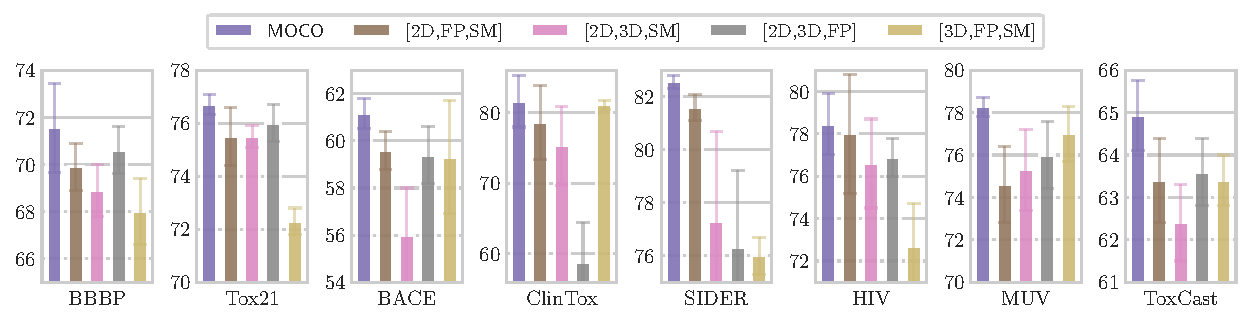
\includegraphics[width=\linewidth]{figures/ablation2.pdf}
	\caption{Ablation studies on four featurization techniques used in \themodel.}
	\label{fig:view-ablation}
\end{figure}

\subsection{Experiments on Variant Fingerprint Encoders}

Since there is a lack of proper neural encoders for fingerprints, we propose an attention-based network to model interactions of feature fields in fingerprint vectors, which considers the discrete and extremely sparse nature of fingerprints.
To demonstrate its effectiveness, we leverage a simple MLP and a Long Short-Term Memory (LSTM) model as the encoder for the fingerprints respectively.
The performance comparison is summarized in \cref{fig:fp-variants}. It is clear that our proposed attention encoder that models feature interactions for fingerprints achieves the best performance.

\begin{figure}
	\centering
	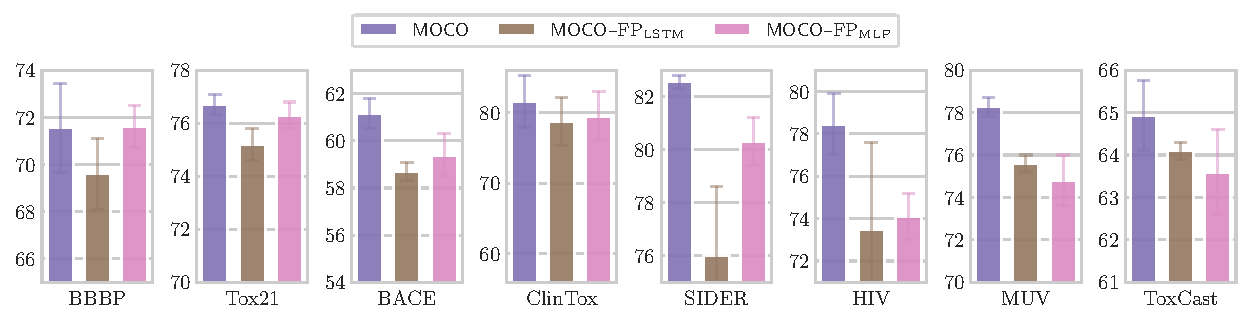
\includegraphics[width=\linewidth]{figures/fpvariants.pdf}
	\caption{Results with two variant encoders for fingerprints: MLP and LSTM.}
	\label{fig:fp-variants}
\end{figure}

\section{More Related Work}
\label{supp:related-work}

The following section provides a more broad literature review across the spectrum of self-supervised representation learning.

\subsection{Self-Supervised Representation Learning on Visual and Natural Language Data}

A SSL model trains itself by learning a part of the input from another through pretext tasks.
Depending on the pretext task, the existing SSL studies can be divided into three main categories.

Early SSL work studies \emph{predictive training} on pseudo-labels directly computed from the raw data.
In Computer Vision (CV) domains, typical pretext tasks include image inpainting \cite{Pathak:2016gb}, rearranging shuffled image patches \cite{Noroozi:2016hd}, colorizing grayscale images \cite{Zhang:2016fr,Larsson:2017vt}, recognizing geometric transformations \cite{Gidaris:2018wr}, and predicting cluster assignments \cite{Caron:2018ba}.
In Natural Language Processing (NLP), word2vec \cite{Mikolov:2013uz} popularizes this paradigm by proposing Continuous Bag-Of-Words (CBOW) and skip-gram models for predicting center and neighboring words, respectively.
Other exemplary work includes \citet{Kiros:2015uq} that predicts neighborhood sentences and BART \cite{Lewis:2020il} that recovers sentence permutation.

The second group of SSL is \emph{contrastive} learning, which seeks to maximize the agreement of embeddings in the latent space under stochastic data augmentations by contrasting positive and negative samples \cite{Jing:2021cf}.
It has revolutionized unsupervised representation learning in recent years \cite{vandenOord:2018ut,Bachman:2019wp,He:2020tu,Chen:2020wj,Caron:2020uv,Chen:2021ci,Gao:2021wf} and has been witnessed to perform on par with its supervised counterparts \cite{He:2020tu,Chen:2020wj}.
A key success to contrastive models is to leverage strong data augmentations that induce invariance irrelevant to properties of the end tasks \cite{Xiao:2021vt,Tian:2020vw,Purushwalkam:2020wm,vonKugelgen:2021wb}.

The third line of development focuses on \emph{generative modeling} of input data.
Its core idea is to randomly remove a portion of data and train the model to recover the removed content.
This so-called masked language modeling and its autoregressive counterparts are first pioneered in the NLP community \cite{Bengio:2003vh,Peters:2018jz,Devlin:2019uk,Liu:2019dd,Lan:2020tt,Radford:2018im,Radford:2019lm,Brown:2020tp} and have since gained increasing popularity in the CV domain \cite{Dosovitskiy:2021uc,He:2022hx,Wei:2021ev}.
Unlike contrastive learning, generative approaches do not rely on curated data augmentations.
It has been reported that they scale well and generalize to different downstream tasks \cite{Devlin:2019uk,Brown:2020tp,He:2022hx}.

\subsection{Graph Self-Supervised Representation Learning}
Analogous to the above studies on visual and natural language data, SSL approaches in the graph domain can also be organized into the same three categories.
Due to the rapid development of graph SSL, we only review the most representative studies in each group.
Readers may refer to recent surveys \cite{Wu:2022wg,Xie:2022uv,Liu:2022wc} for comprehensive reviews and \citet{Zhu:2021tu} for a benchmarking study.

Firstly, the pioneering \emph{predictive} model \citet{Hu:2020uz} explores four strategies at both node and graph levels, including masked attribute prediction, context prediction, supervised attribute prediction, and structural similarity prediction.
\citet{You:2020um} study three SSL tasks through a multi-task framework to enable predictive training of graph-structured data.
M3S \cite{Sun:2020wx} explores the use of cluster assignments \cite{Caron:2018ba} as pseudo-labels and proposes a self-training framework that incrementally adds high-confident nodes to the labeled dataset.

The second group of work studies \emph{generative} training.
GraphSAGE \cite{Hamilton:2017tp} performs the link prediction task to reconstruct the graph structure in a once-for-all manner, similar to graph autoencoders \cite{Kipf:2016ul}.
GPT-GNN \cite{Hu:2020vh} proposes to perform node and edge reconstruction iteratively.

Lastly, along the line of graph \emph{contrastive} learning, some investigate contrasting modes for graph data, typical work of which includes cross-scale contrasting \cite{Velickovic:2019tu,Hassani:2020un}, same-scale contrasting \cite{Sun:2020vi,Zhu:2020vf,You:2020ut}, and hierarchical contrasting \cite{Xu:2021tv,Lin:2021vt}.
Another line of work investigates data augmentations.
GraphCL \cite{You:2020ut} proposes four heuristic augmentation schemes including edge dropping, node dropping, attribute masking, and subgraph cropping; its follow-up JOYO \cite{You:2021wl} proposes to learn the augmentation priors via bi-level optimization.
GCA \cite{Zhu:2021gx} proposes adaptive augmentation that better preserves important semantics and structures of the underlying graph.
SimGRACE \cite{Xia:2022gd} eschews the need of explicit augmentation;
\citet{Trivedi:2022de} propose content-aware augmentation to avoid corrupting task-relevant information.
